\documentclass[a4paper, 12pt]{article}

\usepackage{amsmath}
\usepackage{hyperref}
\usepackage{cleveref}
\usepackage[left=0.6in,right=0.6in]{geometry}
\usepackage{esdiff}

\usepackage{graphicx}
\graphicspath{ {./resources/} }

\begin{document}

\section{Logistic regression and the loss formulation}

Logistic regression (LR) has the following form:

\begin{equation}\label{eq-logistic}
f(x) = \frac{1}{\exp(-(W^T x + b)) + 1}
\end{equation}

Where $x$ is the feature for a sample (shape $1\times D$), W is the weight (shape $1\times D$),
and $b$ is the bias term.

The log loss for a single sample has the following form:

\begin{equation}\label{eq-loss-single}
    loss = -(y\log(1-p) + (1-y)\log(1-p))
\end{equation}

where $y$ is the ground truth label and $p$ is the prediction by LR.

For a batch of $N$ samples, the loss is averaged over the batch:

\begin{equation}\label{eq-loss-batch-no-regu}
    loss = -\frac{1}{N}\sum_{i=1}^{N} y\log(p) + (1-y)\log(1-p)
\end{equation}

If we add L2 regularization for the weight vector, the final loss we are going to minimize is:

\begin{equation}\label{eq-loss-with-regu}
    L = -\frac{1}{N}\sum_{i=1}^{N} y\log(p) + (1-y)\log(1-p) + \alpha \frac{1}{2} {\lVert W \rVert}^2
\end{equation}

$\alpha$ is the term used to control the regularization effect.

\section{Derivative of the loss}

Now let's derive the first part of the loss w.r.t to the weight $W$ for a single sample.

Let

\begin{equation}
    \begin{aligned}
        p &= \frac{1}{e^{-z} + 1} \\
        z &= W^T x + b
    \end{aligned}
\end{equation}


Based on chain rule, the derivative of loss in \cref{eq-loss-single} w.r.t W can be written as:

\begin{equation}\label{eq-deriv-single}
    -\left (y \cdot \frac{1}{p}\cdot \frac{\partial p}{\partial z} \cdot \frac{\partial z}{\partial W} + (1-y)\cdot
        \frac{-1}{1-p}\cdot \frac{\partial p} {\partial z} \cdot \frac{\partial z}{\partial W} \right)
\end{equation}

The partial derivative is:

\begin{equation}\label{eq-partial-deriv}
    \begin{aligned}
        \diffp{p}{z} &= \frac{e^{-z}}{(e^{-z} + 1)^2} = p(1-p)\\
        \diffp{z}{W} &= x
    \end{aligned}
\end{equation}

Now we substitute \cref{eq-partial-deriv} into \cref{eq-deriv-single} and simply it a bit, we get the following:

\begin{equation}\label{eq-partial-single-final}
    (p - y)x
\end{equation}

Now we deal with the regularization part in the loss, the derivative w.r.t to $W$ is easy to get:

\begin{equation}\label{eq-partial-regu}
    \alpha W
\end{equation}

With \cref{eq-partial-single-final} and \cref{eq-partial-regu}, now it is easy to get the derivative of overall $L$
w.r.t $W$:

\begin{equation}\label{eq-deriv-L-to_w-non-matrix}
    \diffp{L}{W} = \frac{1}{N} \sum_{i=1}^{N} (p^{(i)} - y^{(i)}) x^{(i)} + \alpha W
\end{equation}

Actually, we can write the above formulation as matrix form to make it more succinct:

\begin{equation}\label{eq-deriv-L-to_w-matrix}
    \diffp{L}{W} = \frac{1}{N} (\mathbf{P} - \mathbf{Y})^T \mathbf{X} + \alpha W
\end{equation}

In the above equation, both $\mathbf{P}$ and $\mathbf{Y}$ are of shape $N\times 1$,
and $\mathbf{X}$ is of shape $N\times D$.

Similarly, we can derive the derivative of $L$ w.r.t bias $b$:

\begin{equation}\label{eq-deriv-L-to_b-matrix}
    \diffp{L}{b} = \frac{1}{N} (\mathbf{P} - \mathbf{Y})^T \mathbf{I}
\end{equation}

where $I$ is of shape $N\times 1$ and has value of all 1.

\section{Parameter update}

The parameter update rule is:

\begin{equation}\label{eq-param-update-rule}
    \begin{aligned}
        W^{t+1} &= W^{t} - \eta \diffp{L}{W} \\
        b^{t+1} &= b^{t} - \eta \diffp{L}{b}
    \end{aligned}
\end{equation}

In the above equation, $\eta$ is the learning rate.

\section{Implementation and discussions}

Overall structure of the code:

\begin{enumerate}
    \item Load and clean the data
    \item Split the data into train and val, here I use 0.8 for train and 0.2 for val
    \item Augment the train data to make the two classes have balanced samples
    \item Train the model (checkpoint the best model)
    \item Predict on the validation set
\end{enumerate}

The SGDClassifier has been updated to support training the logistic regression and for predicting the result.
See the code for the details.

\subsection{data cleaning}

I used t-SNE for data visualization and find that there is indeed a few samples that can not be clustered well.
The t-SNE code can be found in the jupyter notebook data-vis.ipynb.

\begin{figure}[h]
    \centering
    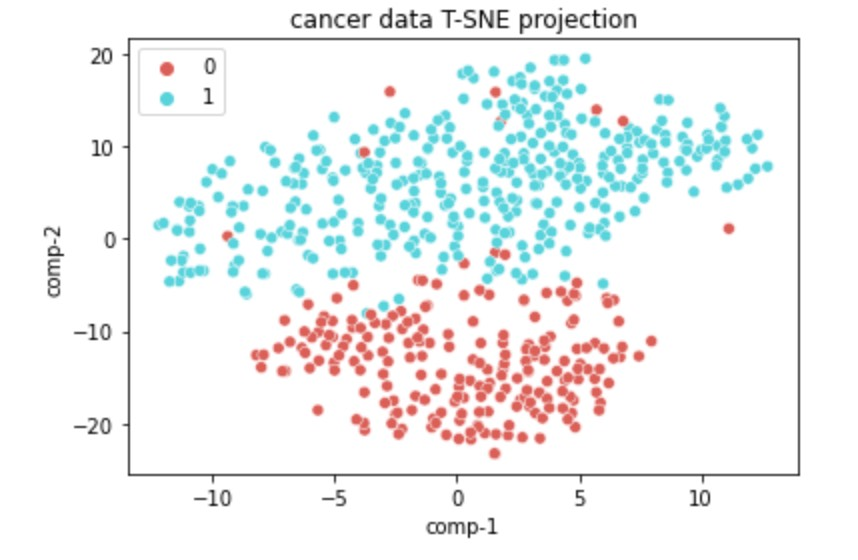
\includegraphics[width=0.75\textwidth]{data-tsne.jpg}
    \caption{data t-SNE visualization}
\end{figure}

Here I only used simple heuristics to find possible noise.
Since the data is relatively clean, to find noise, I simply train the model on the whole dataset.
This will give use a relatively good model for predictions.
Then we use the trained model to predict the probability and class for each sample.
If the class prediction is wrong, but the model has strong confidence
(0.8 if the ground truth is 0, 0.2 if the ground truth is 1),
then this sample is likely to be an outlier.

I have also tried more sophisticated method like LOF or Isolation forest, but find their result less
interpretable and do not match with each other. The code can be found in script det-noise.py.
So I decided to use this simpler way to find outliers.

\subsection{Early stopping}

For early stopping, we usually use the accuracy on validation set as a indicator.
If the accuracy on validation set stops improving for a certain period,
then further training may lead to overfitting of the model.

\subsection{Model performance on unseen dataset}

It depends on the data distribution of unseen data.
If the data distribution on the unseen dataset is similar to that of training set,
then the model will perform reasonably well on unseen data.
Also with the use of weight regularization and dropout, the model should be better at unseen dataset.

\subsection{Impact of lr and batchsize}

If we use a small learning rate,
the model may converge a lower val accuracy or converges slower.
For example, fix batch size to 32, if we use 0.001 as lr, the best val acc is 96.46\%.
If we use 0.01 as lr, the best val acc is 98.23\%, at about epoch 42.
If we use 0.05 as lr, the beat val acc is 99.11\%, at about epoch 22.

If we fix learning rate and change batch size, large batch size may lead to slower convergence,
since the model weight update frequency is lower compared to smaller batch size.
For example, if we use batch size 64, the model gets 99.11\% accuracy at epoch 50.
If we use batch size 128, the model gets the same accuracy at epoch 60.
If we use batch size 300, the model may need more than 200 epochs to reach the same accuracy.

\subsection{Bonus questions}

\begin{enumerate}
    \item Is it possible to modify the training data and learn just the weight vector?\\

    Yes, we can add a feature with value 1 for each sample, then we can drop the bias term.
    Now the new weight we are going to learn is $D + 1$ dimension, where $D$ is the original feature dimension.

    \item Add a function \textbf{\_\_dropout}, which randomly sets some of feature values to zero during training.
        How will you incorporate it during fit / predict? \\

    The dropout function has been added to the SGDClassifier.
    During training, each sample is masked based on the probability $p$.
    We multiply the original feature with the mask, and then divide it by $1-p$.
    Because if we mask the element of each sample with probability $p$,
    then the remained value is roughly only $1-p$ of the original value.
    During test, we just use the unmasked features and predict as is, not modification is needed.

    \item  Does \_\_dropout help in convergence / overfitting ?

    Generally, dropout will help regularize the model and make it do better on testing.
    However, this dataset is so small, even without dropout, we can get high accuracy on val set.

\end{enumerate}

\end{document}
